\section{Observing Magnetic Fields from Electric Currents}

\instructornote{%
Time: 20 minutes for activity 1

Activity 1 of this lab was added by Matt Trawick in 2017.  Need to use very small compasses for this, like about 1~cm across.  With power supplies at their maximum current (3 amps) students can just barely see the effect here.  It would be better if we had slightly larger current supplies.
}

\makelabheader %(Space for student name, etc., defined in master.tex)

\bigskip
\textbf{Apparatus} 

\begin{itemize} [nosep]
\item Power supply
\item Long jumper wire 
\item Lab stand and clamps for holding wire vertically
\item One regular size compass
\item One teeny-weeny compass
\item Tangent Galvanometer
\end{itemize}

\bigskip
\textbf{Activity 1: Magnetic Field Due to Current in a Straight Wire}

Before you do anything else, verify that your teeny-weeny compass actually works.  It should point north when it's far away from any magnets or steel.  

\begin{enumerate}[labparts]

\item Make a prediction: will electric current in a wire produce a magnetic field that will deflect your compass?  If so, what direction will the magnetic field point?  (Radially inwards, towards the wire?  Away from the wire?  Circumferentially around the wire?)  You may not have discussed this in class, but at least take a wild guess.
\answerspace{0.5 in}

Set up your equipment to do the experiment, connecting the power supply so that positive current travels \textit{up} the vertical wire.  Crank the current up all the way so that the display reads just over 3 Amps.  

\item Hold the teeny-weeny compass very close to the vertical section of the wire, so that the outside of the compass  actually \textit{touches} the wire's rubber insulation.  Move the compass on all sides of the wire (in front, behind, etc.).  Based on your observations, describe the apparent direction of the magnetic field near the wire. \label{part_straight_wire_regular}
\answerspace{0.5 in}

\item By pointing north, your compass is pointing \textit{in the direction} of the local magnetic field.  As you look down on the vertical wire from above, does the magnetic field seem to point \textit{clockwise} or \textit{counterclockwise} around the wire? 
\answerspace{0.3 in}

\item Make a prediction: what do you think will happen to the magnetic field when you reverse the direction of the current in the vertical wire, so that current travels \textit{down} instead of \textit{up}? \label{part_straight_wire_reversed}

\bigskip
\hspace{0.5in} Prediction:

\bigskip
\hspace{0.5in} Experiment:
\bigskip

\item The direction of the magnetic field is supposed to obey the following ``right-hand rule:''
\begin{quote}\textit{If you grab a wire with your right hand, with your thumb pointing in the direction of the current, your fingers should wrap around the wire in the direction of the magnetic field.}
\end{quote}
Are the results of your experiments in parts \ref{part_straight_wire_regular} and \ref{part_straight_wire_reversed} both consistent with this right-hand rule?
\answerspace{0.3 in}

\end{enumerate}

\textbf{Activity 2: Magnetic Field Due to Current in a Circular Coil}

In this investigation we will use a device known as a tangent galvanometer to make a qualitative study of the effect of current (moving charges) in a coil of wire on a compass. A sketch of the galvanometer is shown below.

\begin{center}
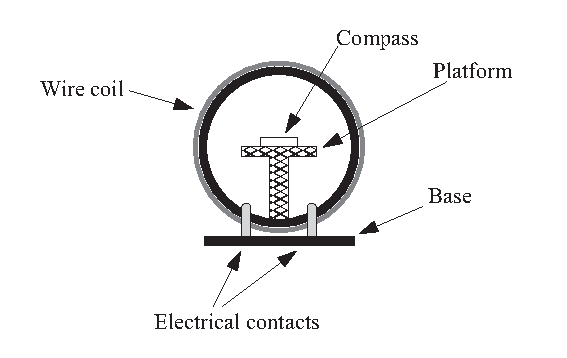
\includegraphics{magnetism_currents/tangent_galvanometer_bw.eps}
\par
Figure 1. Tangent galvanometer and compass.
\end{center}

\begin{enumerate}[labparts]
\item With the power supply off, connect the positive and negative terminals 
on the power supply to the two side screws on the tangent galvanometer. Turn 
the coarse current control on the power supply all the way up and the voltage 
controls all the way down.

\item Before turning the power supply on, place the compass on the platform 
in the center of the tangent galvanometer. Rotate the galvanometer until the 
compass needle is aligned with the plane of the wire coil of the galvanometer.
Turn the power supply on and slowly turn up the fine voltage control.
What do you observe? Make a sketch to show the orientation of the compass 
needle and galvanometer coil with the voltage on and off. 
(It may be easiest to do this with TOP views.)
\vspace{20mm}

\item Turn the voltage on the power supply to zero.
Rotate the entire setup (galvanometer, compass, wires) $180^\circ$
so the contacts are on the opposite side from where they were before.
Make sure the compass needle is again aligned with the plane of the wire coil.
Slowly turn the voltage back up. What do you observe?
Make another sketch to show the orientation of the compass needle and
galvanometer coil with the voltage on and off.
\vspace{30mm}

\item The deflection of the compass when current flows in the tangent 
galvanometer implies the current creates a magnetic field.
From your observations can you tell the direction
of the magnetic field?  Explain.
\vspace{30mm}

\item Reverse the wires on the contacts of the tangent galvanometer to reverse 
the direction of the current in the coil of the galvanometer.
We will now repeat the observations from above.
With the voltage off, align the compass needle and the plane of the wire coil 
of the galvanometer as in part (b) above.
Slowly turn up the voltage.
What do you observe?
Make a sketch to show the orientation of the compass and
galvanometer coil with the voltage on and off.
\vspace{30mm}

\item Rotate the entire setup (galvanometer, compass, wires) $180^\circ$
so the contacts are on the opposite side from where they were before.
Make sure the compass needle is again aligned with the plane of the wire coil.
Slowly turn the voltage back up. What do you observe?
 Make another sketch.
\vspace{30mm}

\item Based on your observations, what happens to the magnetic field of the 
tangent galvanometer when you reverse the direction of the current?

\end{enumerate}

